\section{动画变换}\label{sec:动画变换}
\begin{remark}
    本节含有高级内容,第一次阅读时可以跳过。
\end{remark}

\begin{figure}[htbp]
    \centering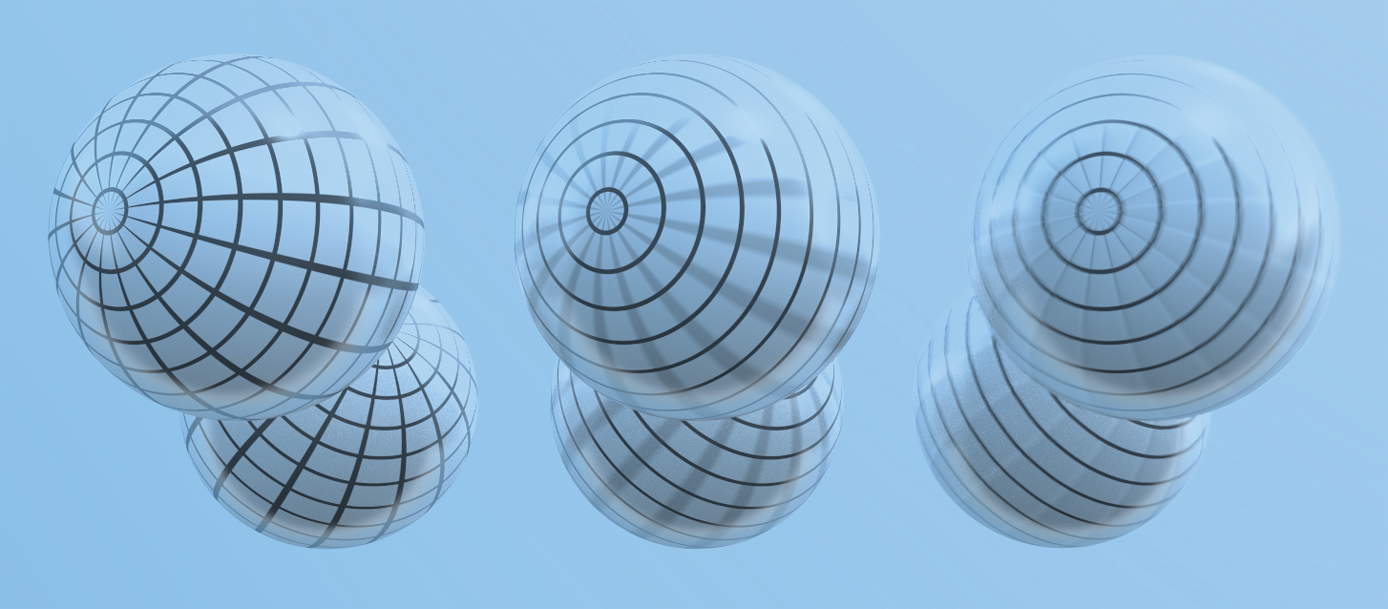
\includegraphics[width=\linewidth]{chap02/spinningspheres.png}
    \caption{转动的球体。用本节实现的变换动画代码以不同速率旋转三个球体并被镜子反射。
        注意球体的反射和球体自身一样模糊。}
    \label{fig:2.15}
\end{figure}

pbrt为场景中的相机和几何图元支持关键帧矩阵动画。
不只是提供单个变换放置场景中的相应物体,
用户还可能提供许多\keyindex{关键帧}{keyframe}{}变换,
每个都与特定时间点关联。
这能让相机移动起来并在仿真相机快门打开时让场景中的物体也移动起来。
\reffig{2.15}展示了三个运用pbrt关键帧矩阵动画的运动球体。

通常,在关键帧矩阵之间插值的问题是没有定义的。
例如,如果我们关于$x$轴旋转181度后再旋转181度,
这代表2度的小旋转还是-358度的大旋转?
再例如,考虑两个矩阵,一个是恒等的另一个是绕$z$轴旋转180度。
从其中一个到另一个有无数种方式可走。

关键帧矩阵插值在计算机动画中是一个重要的问题,
有许多不同的方法被开发出来。
幸运的是,有两个原因使得渲染器中的矩阵插值问题一般不像动画系统中的那么难。

首先,在一个像pbrt那样的渲染器中,
我们一般有分别在相机快门打开和关闭时的关键帧矩阵;
我们只需要在单张图像的时段里在两者之间插值。
在动画系统中,矩阵一般按更低的时间频率提供,
所以一对关键帧矩阵之间有许多帧;
这样,就有更多机会注意到插值中的问题。

第二,在基于物理的渲染器中,需要我们插值的矩阵对的时段越长,
虚拟相机快门就打开得越久,最终图像的运动模糊就越多;
运动模糊的增加常常隐藏了插值的缺点。

对由关键帧矩阵定义的变换最简单的插值方法——
直接对矩阵的每个分量插值——并不是一个好办法,因为它一般会导致意外不良结果。
例如,如果变换应用了不同的旋转,则即使是刚体运动,中间的矩阵也可能缩放物体,这明显不是我们期望的。
(如果矩阵在它们之间有完整180度的旋转,则插值的中间物体可能缩小到不见!)

\reffig{2.16}展示了在该帧过程中旋转90度的球体;
直接对矩阵元素插值给出的结果不如本节实现的方法准确。
\begin{figure}[htbp]
    \raggedright
    \subfloat[静止球体。]{\label{fig:2.16.1}
\includegraphics[width=0.5\linewidth]{chap02/sphere-still.png}}%
    \subfloat[旋转,正确插值。]{\label{fig:2.16.2}
\includegraphics[width=0.5\linewidth]{chap02/sphere-rot-good.png}}\\%
    \subfloat[旋转,错误插值。]{\label{fig:2.16.3}
\includegraphics[width=0.5\linewidth]{chap02/sphere-rot-bad.png}}\quad%
    \begin{minipage}{0.45\textwidth}
        \vspace{-\linewidth}\caption{变换插值错误的影响。(a)球体以网格线作为纹理,没有旋转。
            (b)球体在该帧过程中旋转90度,使用本节实现的变换插值技术。
            (c)球体旋转90度,直接对矩阵分量插值来对变换插值。
            这时,动画球体错误地变大了并且靠球体外本应清晰的线条也错误地变模糊了。}
        \label{fig:2.16}
    \end{minipage}
\end{figure}

pbrt中使用的变换插值方法是基于\keyindex{矩阵分解}{matrix decomposition}{}——
给定任意变换矩阵$\bm M$,我们将其分解为
缩放($\bm S$)、旋转($\bm R$)和平移($\bm T$)变换的级联,
\begin{align*}
    \bm M=\bm S\bm R\bm T\, ,
\end{align*}
其中这些分量每一个都是独立插值,然后合成的插值矩阵由三个插值矩阵一起相乘得到。